\documentclass{article}
\usepackage[utf8]{inputenc}
\usepackage[T2A]{fontenc}
\usepackage[utf8]{inputenc}
\usepackage{float}
\usepackage[russian]{babel}
\usepackage[a4paper, left=10mm, right=10mm, top=20mm, bottom=20mm]{geometry}
\usepackage{natbib}
\usepackage{graphicx}
\usepackage{tabularx}
\usepackage{hyperref}

\title{PSD@CBM firmware description (draft, for personal use)}
\author{Finogeev Dmitry, INR RAS}





\begin{document}

\maketitle

Actual version of the document is avaliable at github:
\newline
\url{https://github.com/dfinogee/PSD-readout-manual/raw/main/PSD_readout_manual.pdf}



\tableofcontents

\newpage

\section{ADC data processing}

\subsection{Channel data collecting}
Each channel collect data in FIFO in hit packet format and emite ready signal after data pushed. Ready signal is syncronious to signal treshold crossing and used for event ADC timestamp ~\ref{fig:1}.


\begin{figure}[H]
	\centering 
	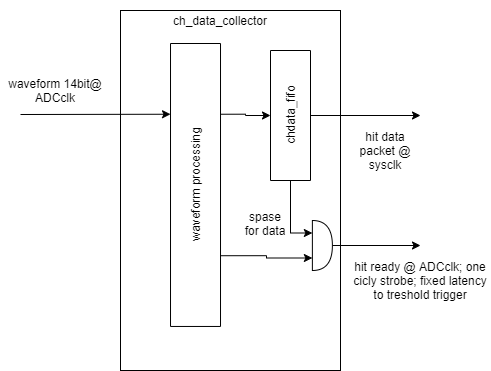
\includegraphics[width=0.5\textwidth]{ADC_event_collection.png}
	\caption{\label{fig:1} Data collecting scheme for single channel}
\end{figure}




\end{document}

